\chapter{Not Gate}
%\stepcounter{chapter}

Con el objetivo de implementar una compuerta \emph{NOT} utilizando transistores de tegnología \emph{BJT}, se optó por investigar el diseño de dicha compuerta para un transistor \emph{NPN} y para uno \emph{PNP}.
Finalmente se obtuvieron los siguientes diseños para lograr una compuerta \emph{NOT}:

\begin{center}
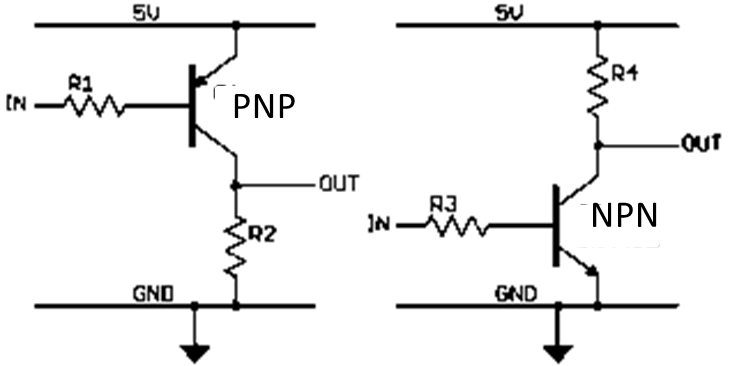
\includegraphics[scale=1]{../1-NotGate/circuitos.png}
\end{center}

El comportamiento lógico de la compuerta \emph{NOT} se muestra en la siguiente tabla de verdad:
\begin{center}
Tabla de verdad NOT GATE
	\begin{center}
		\begin{tabular}{|c|c|}
					\hline
					\textbf{INPUT} & \textbf{OUTPUT} \\
					\hline
					0  &  1\\
					\hline
					1  & 0\\
					\hline
				\end{tabular}
	\end{center}
\end{center}

\section{Mediciones}
Una vez armado ambos circuitos, se procedió a realizar las correspondientes mediciones:
\begin{center}
Mediciones NOT GATE con transistor NPN
	\begin{center}
		\begin{tabular}{|c|c|c|}
					\hline
					\textbf{} & \textbf{sin capacitor} & \textbf{con capacitor}\\
					\hline
					\textbf{High-level input voltage (VIH)} & 4.93V & 4.93V\\
					\hline
					\textbf{Low-level input voltage (VIL)} & 70mV & 	70mV\\
					\hline
					\textbf{High-level output voltage (VOH)} & 5.05V & 5.05V\\
					\hline
					\textbf{Low-level output voltage (VOL)} & 10mV & 10mV\\
					\hline
					\textbf{High-Noise Margin} & 0.12mV & 0.12mV\\
					\hline
					\textbf{Low-Noise Margin} & 0.06V & 0.06V\\
					\hline
					\textbf{Propagation delay High-to-Low} & 41.8nS & 81nS\\
					\hline
					\textbf{Propagation delay Low-to-High} & 2.98uS & 4.41uS\\
					\hline
					\textbf{Transition time High-to-Low} & 64nS & 94nS\\
					\hline
					\textbf{Transition time Low-to-High} & 346nS & 2.98uS\\
					\hline
				\end{tabular}
	\end{center}
\end{center}
\begin{center}
Mediciones NOT GATE con transistor PNP
	\begin{center}
		\begin{tabular}{|c|c|c|}
					\hline
					\textbf{} & \textbf{sin capacitor} & \textbf{con capacitor}\\
					\hline
					\textbf{High-level input voltage (VIH)} & 5.04V & 5.04V\\
					\hline
					\textbf{Low-level input voltage (VIL)} & 210mV & 170mV\\
					\hline
					\textbf{High-level output voltage (VOH)} & 5.1V & 5.1V\\
					\hline
					\textbf{Low-level output voltage (VOL)} & 0V & 0V\\
					\hline
					\textbf{High-Noise Margin} & 210mV & 170mV\\
					\hline
					\textbf{Low-Noise Margin} & 0.06V & 0.06V\\
					\hline
					\textbf{Propagation delay High-to-Low} & 670nS & 1.26uS\\
					\hline
					\textbf{Propagation delay Low-to-High} & 400nS & 910nS\\
					\hline
					\textbf{Transition time High-to-Low} & 1.365uS & 1.84uS\\
					\hline
					\textbf{Transition time Low-to-High}	& 810nS & 1.96uS\\
					\hline
				\end{tabular}
	\end{center}
\end{center}
\subsection{Conclusiones}
A través de las mediciones se puede observar que la compuerta NOT utilizando NPN es más rápida que la de PNP en "Propagation delay High-to-Low" pero pasa lo contrario en "Propagation delay Low-to-High". Y mirando los tiempos de transición, se puede ver que con el NPN son más cortos que con el PNP.
			
%https://www.youtube.com/watch?v=XpN0IQMHo7k
